\chapter{Data}
\label{ch:data}

\section{Choice of database}

A central constraint of this work was to use only data that are \emph{openly licensed,
downloadable and verifiable} by any examiner. Commercial process databases (e.g.\ ecoinvent) were
therefore excluded. AGRIBALYSE (ADEME and INRAE, France) \citep{agribalyse2020,agribalyse31} was
selected because it is (i) published under the French open licence (Licence Ouverte/Etalab);
(ii) product-level, i.e.\ it reports finished-food impacts that can serve directly as
supervised-learning targets; (iii) computed with one consistent method (EF~3.0) and system
boundary; and (iv) accompanied by recipe and life-cycle-stage breakdowns.

\section{Source files}

Three CSV tables of AGRIBALYSE~3.1 were downloaded from the ADEME open-data portal (via
\texttt{data.gouv.fr}) on 5~November~2026:

\begin{table}[ht]
\centering\small
\caption{AGRIBALYSE 3.1 tables used.}
\label{tab:files}
\begin{tabularx}{\textwidth}{@{}lrrX@{}}
\toprule
Table & Rows & Columns & Content and use \\
\midrule
Synthèse (synthesis) & 2{,}451 & 32 & One row per product: names (FR/EN), food group and sub-group,
delivery mode, packaging data source, consumer preparation, season and air-freight flags, Data
Quality Rating (DQR), 16 EF~3.0 indicators + single score. \textbf{Targets and main features.} \\
Détail par ingrédient & 8{,}882 & 24 & Recipe ingredients of composite products. \textbf{Only the
\emph{presence} of each ingredient is used} (its impact columns are never used). \\
Détail par étape & 2{,}451 & 131 & Impacts split by life-cycle stage. \textbf{Descriptive analysis
only}, never a model input. \\
\bottomrule
\end{tabularx}
\end{table}

\section{Cleaning}

\begin{itemize}
  \item The synthesis file contains $\sim$12{,}500 empty trailing rows; these were dropped,
        leaving exactly 2{,}451 products with complete impact values.
  \item Category labels were stripped of whitespace (e.g.\ \texttt{"Four "} vs \texttt{"Four"})
        and translated to English for presentation; the 61 sub-group labels have an
        English display map.
  \item The French category \emph{``Pas de préparation''} is stored as \texttt{No preparation};
        storing it as \texttt{None} would be silently parsed as missing by \texttt{pandas}.
  \item In the ingredient table the pseudo-ingredient \emph{``Autres étapes''} (other steps) was
        removed, giving 5{,}062 product--ingredient links over 286 distinct ingredients and
        1{,}094 composite products.
  \item For log-scale modelling of other impact categories, products with non-positive values
        were excluded for that indicator only: 34 for land use (soil-carbon credits) and 1 for
        water use.
\end{itemize}

\section{The no-leakage rule}

The stage table and the per-ingredient impacts \emph{add up to} the target. A model given these
would trivially reproduce the answer and would be useless in practice, because an analyst who
already has them has already done the LCA. All features were therefore restricted to information
available \emph{before} an LCA: product name, category, storage/delivery mode, consumer
preparation, packaging data source, season and air-freight flags, and the list (not the masses) of
recipe ingredients.

\section{Exploratory analysis}

\subsection{Distribution of the target}

Climate-change impact ranges from 0.0003~kg~\co/kg (tap water) to 52.5~kg~\co/kg (lamb), with
median 2.78 and mean 5.76: the distribution is strongly right-skewed and spans five orders of
magnitude (Figure~\ref{fig:dist}, Table~\ref{tab:groups}). All models are therefore trained on
$y = \log_{10}(\text{GWP})$, which turns multiplicative errors into additive ones and prevents a few
high-impact meats from dominating the loss.

\begin{figure}[ht]
\centering
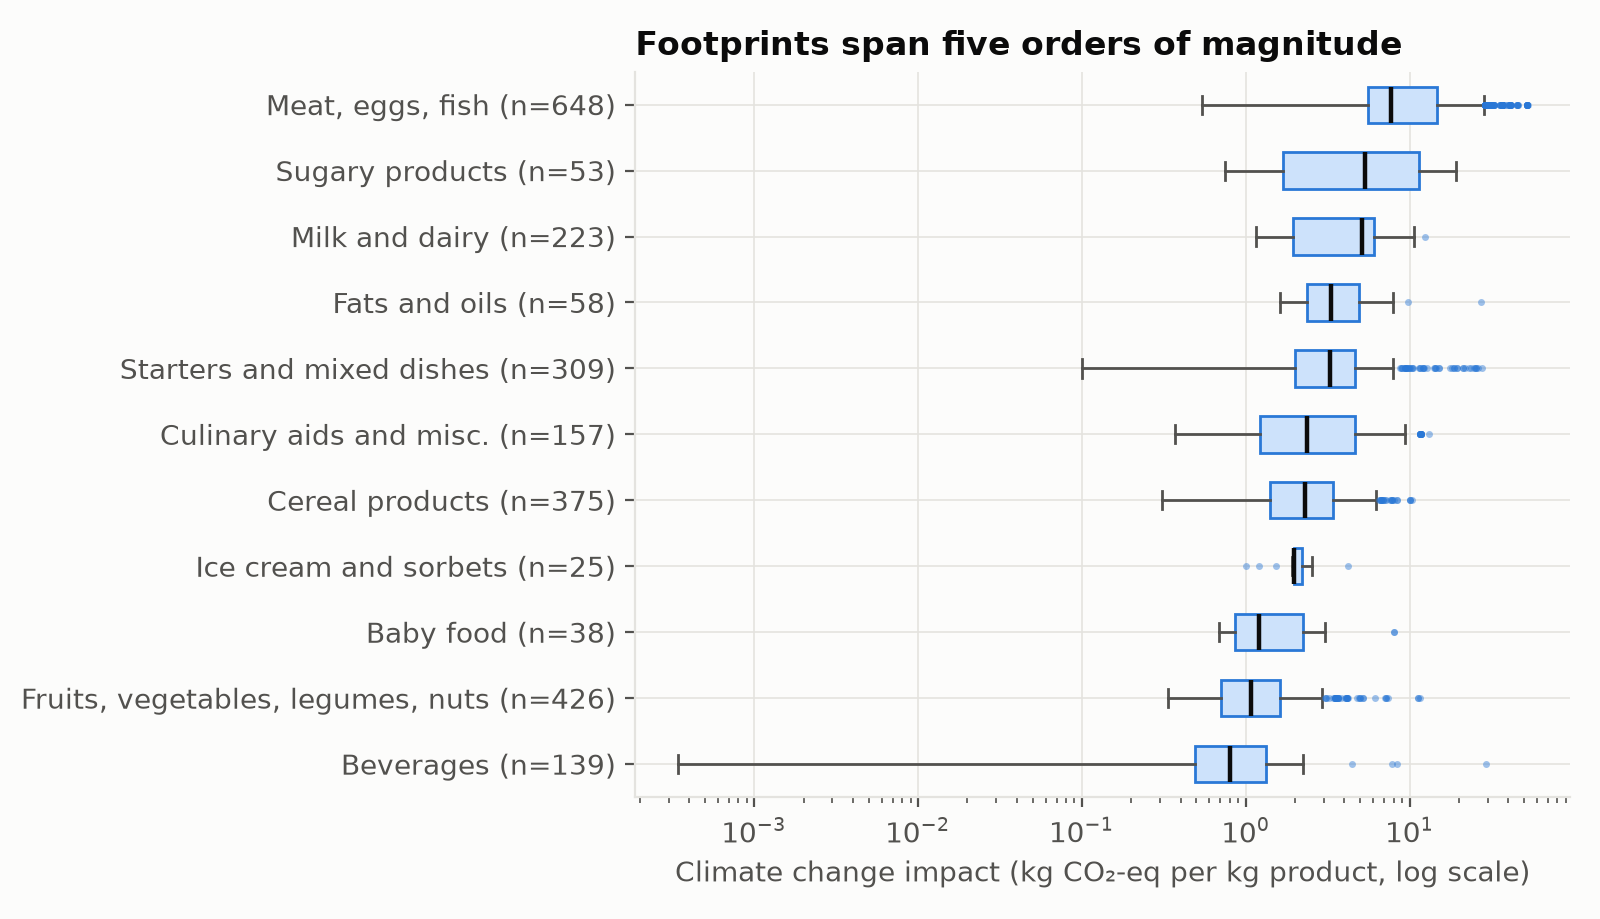
\includegraphics[width=\textwidth]{f1_gwp_by_group}
\caption{Climate-change impact per kg by food group (log scale). Boxes show the inter-quartile range; dots are individual products.}
\label{fig:dist}
\end{figure}

\begin{table}[ht]
\centering\small
\caption{Products and climate impact (kg \co/kg) by food group.}
\label{tab:groups}
\begin{tabular}{@{}lrrrrr@{}}
\toprule
Food group & $n$ & Median & Min & Max & Composite (\%) \\
\midrule
Meat, eggs, fish & 648 & 7.75 & 0.54 & 52.50 & 19 \\
Fruits, vegetables, legumes, nuts & 426 & 1.08 & 0.33 & 11.60 & 12 \\
Cereal products & 375 & 2.30 & 0.31 & 10.30 & 81 \\
Starters and mixed dishes & 309 & 3.26 & 0.10 & 27.80 & 92 \\
Milk and dairy & 223 & 5.16 & 1.15 & 12.50 & 31 \\
Culinary aids and misc. & 157 & 2.37 & 0.37 & 13.20 & 48 \\
Beverages & 139 & 0.80 & 0.0003 & 29.10 & 47 \\
Fats and oils & 58 & 3.30 & 1.63 & 27.40 & 28 \\
Sugary products & 53 & 5.32 & 0.75 & 19.30 & 87 \\
Baby food & 38 & 1.21 & 0.68 & 8.05 & 100 \\
Ice cream and sorbets & 25 & 1.98 & 1.00 & 4.24 & 100 \\
\midrule
\textbf{All} & \textbf{2,451} & \textbf{2.78} & \textbf{0.0003} & \textbf{52.50} & \textbf{45} \\
\bottomrule
\end{tabular}
\end{table}

Two observations matter for modelling. First, \emph{between-group} differences are large (median
meat footprint is seven times that of fruit and vegetables), so category information alone is
valuable. Second, \emph{within-group} spread is also large (a factor of 100 within meat), so
category averages are insufficient -- finer product information is required.

\subsection{Where in the life cycle do impacts arise?}

Figure~\ref{fig:stages} aggregates the stage table by food group. Agriculture dominates for
animal products (88\% for meat, eggs and fish; 79\% for dairy), while packaging and transport
become significant for beverages and fruit and vegetables. Since agricultural impact is driven
mainly by \emph{what} the food is (species, crop), this suggests that product identity --
captured by its name and ingredients -- should be the most informative feature, which is
confirmed in Section~\ref{sec:ablation}.

\begin{figure}[ht]
\centering
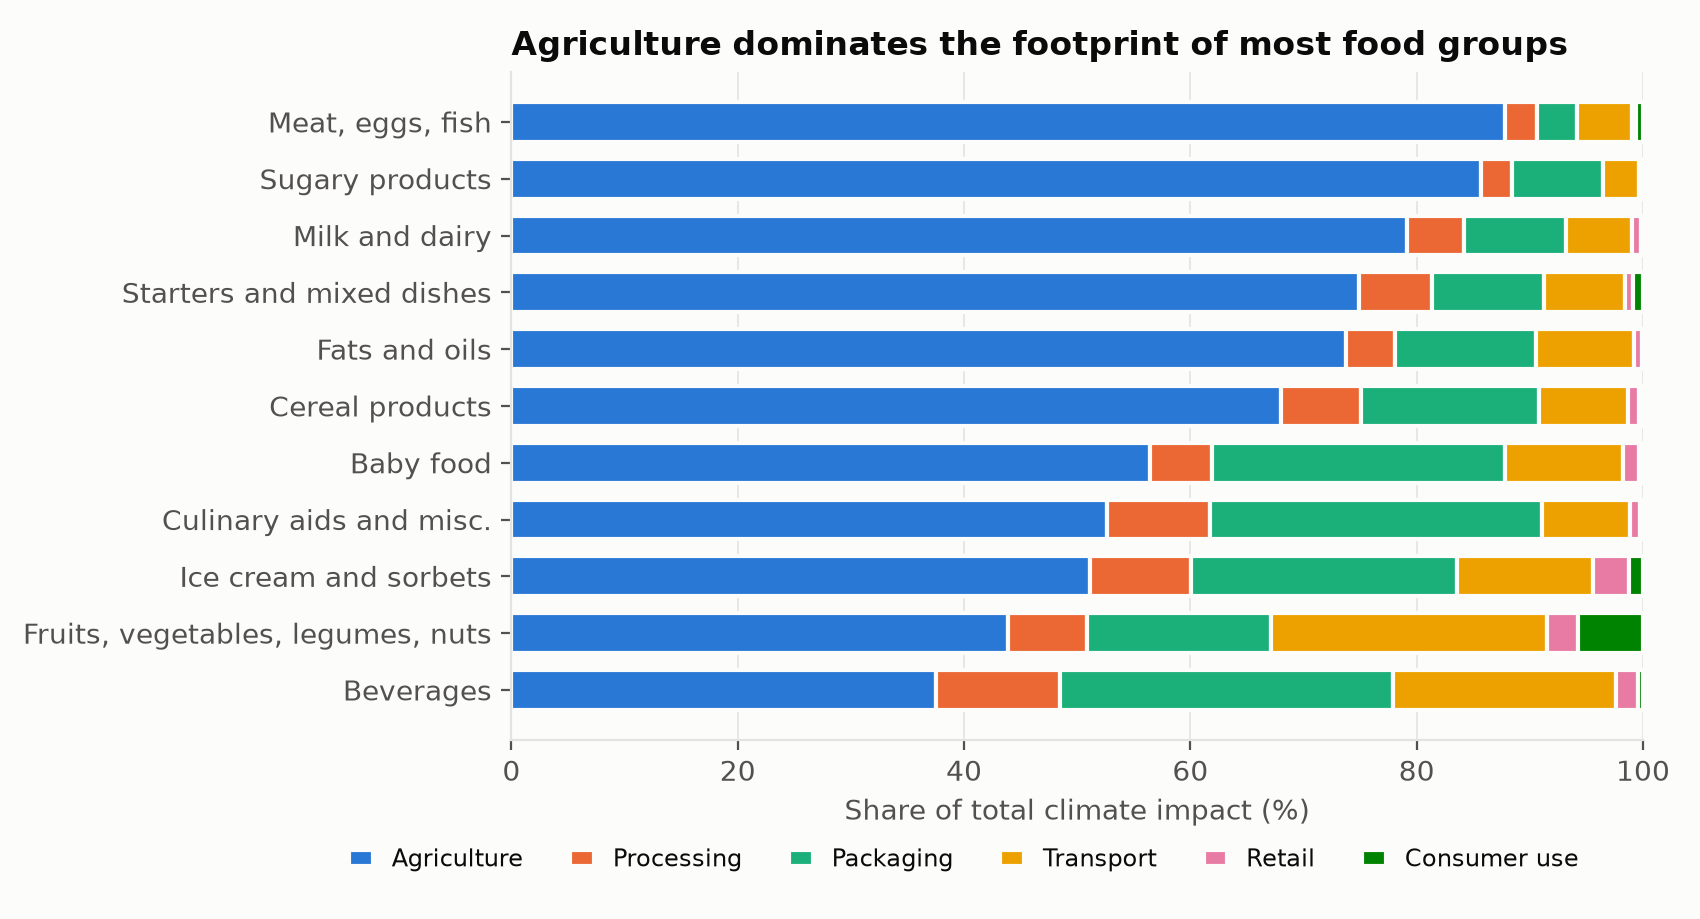
\includegraphics[width=\textwidth]{f2_stage_contribution}
\caption{Share of climate impact by life-cycle stage and food group (descriptive only; never a model input).}
\label{fig:stages}
\end{figure}

\subsection{Categorical descriptors}

Delivery mode: chilled 1{,}223, ambient long shelf-life 821, ambient medium 238, frozen 97,
ambient short 72. Consumer preparation: none 1{,}646, oven 300, microwave 262, boiling 119,
pan-frying 72, refrigerated at home 52. Packaging data come from AGRIBALYSE-specific data for
1{,}284 products and from proxies for 1{,}167. The mean Data Quality Rating is 2.46
(1 = best, 5 = worst), indicating generally good but heterogeneous underlying data quality.
Season and air-freight flags are almost constant (only 4 and 2 exceptions), so they carry little
information.
